\documentclass{beamer}
\usetheme{Warsaw}
\setbeamertemplate{headline}{}
\graphicspath{ {./images/} }
\usepackage{amsmath}

\usepackage{amssymb}
\usepackage{algpseudocode}
\usepackage{algorithm}
\usepackage{setspace}
\usepackage{graphicx}
\usepackage{hyperref}
\usepackage{siunitx}
\usepackage{amsmath}
\usepackage{caption}
\usepackage{subcaption}

\usepackage{amssymb}
\usepackage{algpseudocode}
\usepackage{algorithm}
\usepackage{setspace}
\usepackage{graphicx}
\graphicspath{ {./images/} }
\usepackage{hyperref}
\usepackage{siunitx}
\usepackage{amsmath}
\usepackage{caption}
\usepackage{subcaption}
\usepackage{geometry}
\usepackage[english]{babel}
\usepackage[T1]{fontenc}
\usepackage[utf8]{inputenc}


\usepackage{tikz}
\usetikzlibrary{positioning}
% \usetikzlibrary{graphdrawing.trees}

\usepackage{booktabs}

\title[HPO using RL Surrogates]{Hyperparameter Optimization using Ranking Loss Surrogates}

\institute{
    {Albert-Ludwigs-University Freiburg
    \\Representation Learning Department}
}

\author[Abdus Salam Khazi]
{
    {Master's Thesis}\\
    {by} \\
    Abdus Salam Khazi
}

\iffalse
\institute{Supervisors: \\
            \begin{tabular}{ll}
		    	JProf. Josif Grabocka \& Sebastian Pineda
		    \end{tabular}
}
\fi

\date{\today}
\logo{
\includegraphics[width=.2\textwidth]{Logo}}

\hypersetup{
    colorlinks=false,
    linkcolor=blue,
    filecolor=magenta,      
    urlcolor=cyan,
}

\begin{document}

\begin{frame}
\titlepage
\end{frame}

\begin{frame}{Table of Contents}
\tableofcontents
\end{frame}

\section{Introduction}
\begin{frame}

\centering
\LARGE{Introduction}

\end{frame}

\begin{frame}[t]{Hyperparameter Optimization (HPO)}
What is HPO?
\begin{itemize}
\item Machine Learning (ML) is a method of learning a parametric model to approximate an unknown function with the help of data.
\item Learning an ML model is the process of learning the parameters of the parametric model.
\item Hyperparameters are variables that help in the process of learning.  E.g., Learning rate,  regularization type.
\item Optimization of the hyperparameters is called HPO.
\end{itemize}

Why is HPO important?
\begin{itemize}
\item ML models are very sensitive to their Hyperparameters (HP).
\item Selecting a good HP configuration is essential to\\
 squeeze out most of the performance from the \\
 ML model.

\end{itemize}

\end{frame}


\begin{frame}[t]{HPO Definition}

HPO can be seen as selecting a hyperparameter setting to obtain the best (lowest) validation error during ML training.
Mathematically,  HPO objective can be defined as:

$$
\underset{\rm \textbf{x}}{\rm argmin} \;\; f(m^{trained}_{\textbf{x}}(\textrm{Data}_{\textrm{val}})) \mapsto \mathbb{R}  \;\;  \forall \textbf{x} \in \mathbb{S}
$$

where
\begin{itemize}
\item $\textbf{x}$ is a HP configuration.
\item $\mathbb{S}$ is the HP search space.
\item $f$ is the evaluation criterion. (Different for Regression,  Classification, etc.)
\item $m^{trained}_{\textbf{x}}$ is a model trained with '$\textbf{x}$' HP configuration.
\item $\textrm{Data}_{\textrm{val}}$ is the validation split of the data.
\end{itemize}

\end{frame}

\begin{frame}[t]{HPO Constraints}

HPO problem has the following unique constraints:

\begin{itemize}
\item It is a non-convex optimization problem.
\item The objective function $f$ is stochastic.
\item Variables (dimensions) may be conditionally dependent on others.  E.g.,  neurons in a layer are conditioned on the existence of the layer.
\item Variables (dimensions) maybe discrete or continuous.
\end{itemize}

We target HPO of discrete HP search spaces.

\end{frame}

\section{Related Work}

\begin{frame}

\centering
\LARGE{Related Work}

\end{frame}

\begin{frame}[t]{HPO Solutions}
Various types of solutions to the HPO problem are proposed:
\begin{itemize}
\item \textbf{Blackbox HPO}: $f$ is treated as a blackbox function. E.g. Random Search, Grid search.
\item \textbf{Online HPO}: Hyperparameters and parameters of an ML model are trained together. E.g., Interleaved updating of the HP and parameters. 
\item \textbf{Multi-fidelity HPO}: Cheap approximations of the HPO objective functions called surrogates/fidelities are used.
E.g. Successive halving.
\item \textbf{Transfer Learning HPO}: Cheap Surrogates are meta learned using existing metadata.
The meta-knowledge is transferred to the target HPO task. 
E.g.  Few Shot Bayesian Optimization (FSBO).
\end{itemize}
\end{frame}

\begin{frame}[t]{HPO Solutions - SMBO}

\textbf{SMBO} - Sequential Model based Optimization. The following steps are performed in a chronologically:

\begin{itemize}
\item From known data $D = {(x_1, f(x_1)), (x_2, f(x_2)), (x_3, f(x_3)) .... }$, build a probabilistic surrogate model of the objective function.
\item Use the surrogate and an acquisition function to sample the next best HP configuration $x'$. Evaluate $f(x')$.
\item Append $(x', f(x'))$ to $D$ and repeat the process.
\end{itemize}

\textbf{Our Research}:

\begin{itemize}
\item We propose the usage the concept of ranking when learning a surrogate using $D$.
\item We propose a context aware surrogate design.
\item Our proposed method is a Transfer HPO method.
\end{itemize}
\end{frame}


\section{Baselines}
\begin{frame}

\centering
\LARGE{Baselines}

\end{frame}

\begin{frame}[t]{Deep Ensembles}

\begin{itemize}
\item Used as non transfer surrogates in SMBO algorithm.
\item It is an ensemble of neural networks.
\end{itemize}

\begin{figure}[H]
\centering
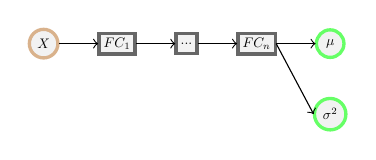
\begin{tikzpicture}[scale=0.5, transform shape,
roundnode/.style={circle, draw=brown!60, fill=black!5, very thick, minimum size=7mm},
roundnodey/.style={circle, draw=green!60, fill=black!5, very thick, minimum size=7mm},
squarednode/.style={rectangle, draw=black!60, fill=black!5, very thick, minimum size=5mm},
]
%Nodes
\node[roundnode]      (X)                             {$X$};
\node[squarednode]      (FC1)                      [right=of X]        {$FC_1$};
\node[squarednode]      (FCmiddle)             [right=of FC1]        {...};
\node[squarednode]      (FCn)                      [right=of FCmiddle]        {$FC_n$};
\node[roundnodey]      (mean)                             [right=of FCn] {$\mu$};
\node[roundnodey]      (variance)                             [below=of mean] {$\sigma^2$};

%Lines
\draw[->] (X.east) -- (FC1.west);
\draw[->] (FC1.east) -- (FCmiddle.west);
\draw[->] (FCmiddle.east) -- (FCn.west);
\draw[->] (FCn.east) -- (mean.west);
\draw[->] (FCn.east) -- (variance.west);
\end{tikzpicture}
\caption{Architecture of a single neural network.}
\label{fig:undividedarchitecture}
\end{figure}

\begin{itemize}
\item Training can be done in parallel.
\item They are reinitialized at every SMBO step.
\item Loss function used to train the neural networks ($\sigma^2$ is variance and $\mu$ is the mean):
\end{itemize}

$$
L_{de} = \frac{\log \sigma^2 }{2} + \frac{(y - \mu)^2}{2\sigma^2} + k
$$

\end{frame}

\begin{frame}[t]{FSBO}
FSBO - Few Shot Bayesian Optimization.
\begin{itemize}
\item It is a state of the art transfer HPO method.
\item Formulates HPO problem as a few shot learning task.
\item Uses deep kernels as surrogates which are of the form:
$$
k(\phi(\textbf{x}, \textbf{w})  ,   \phi(\textbf{x'}, \textbf{w}) |  \mathbf{\theta})
$$
where $\textbf{x}$ and $\textbf{x'}$ are HP configurations. $\mathbf{\theta}$ and $\textbf{w}$ are parameters of kernel $k$ and the neural network $\phi$ respectively.

\item The following are done in a chronological steps
\begin{itemize}
\item Meta-training using existing meta data.
\item Fine-tuning for few epochs i.e few shot learning.
\end{itemize}
\item The loss function maximises the following log probability
$$
\log p( \textbf{y}^{(1)}...\textbf{y}^{(T)} | \textbf{X}^{(1)}...\textbf{X}^{(T)}, \mathbf{\theta}, \textbf{w})
$$

\end{itemize}

\end{frame}

\section{Proposed Method: Background}

\begin{frame}

\centering
\LARGE{Proposed Method: Background}

\end{frame}

\begin{frame}[t]{Understanding Ranking}
Consider a set:
$$
\mathbb{A} = \{a_1,  a_2,  a_3, ... ,  a_n\}
$$
If lower rank is better,  then ranking defines an ordering of the elements in $\mathbb{A}$ such that:
$$
\texttt{Rank}(a_i) < \texttt{Rank}(a_j) \iff a_i  \succ a_j
$$

Ranking can be divided into following components
\begin{itemize}
\item Obtaining relevance scores of objects in the set $\mathbb{A}$.
\item Sorting objects based on relevance scores.
\end{itemize}

Since sorting is not differentiable trivially,  we only to model the scoring function $s$ by our ML model.

$$
s : \mathbb{A} \mapsto \mathbb{R}
$$

\end{frame}

\begin{frame}[t]{Understanding Ranking Losses}

Consider that data is given in the following format:

\begin{table} [ht]
\centering
\begin{tabular}{ | c | c | c | }
  \toprule
  Instance & Object Set & Ground Truth \\ \midrule
% \hline \hline
  1 & $\{a_1, a_2, a_3, ... , a_{10}\}$  & $\{y_1, y_2, y_3, ... , y_{10}\}$  \\
  2 & $\{a'_1, a'_2, a'_3, ... , a'_{15}\}$ & $\{y'_1, y'_2, y'_3, ... , y'_{15}\}$  \\
  3 & $\{a''_1, a''_2, a''_3, ... , a''_{7}\}$ & $\{y''_1, y''_2, y''_3, ... , y''_{7}\}$  \\
  ... & $\{...\}$ & $\{...\}$ \\
  \bottomrule
\end{tabular}
\caption{Data used to train a scoring function.}
\label {tab:dataformat}
\end{table}

How do learn the scoring function $s$?
\begin{itemize}
\item Use a parametrized model $s_{\theta}$.
\item Use a (ranking) loss function to get the optimum $\theta^*$.
\end{itemize}

\end{frame}


\begin{frame}[t]{Understanding Ranking Losses}
Types of ranking:
\begin{itemize}
\item \textbf{Pointwise} - The model directly predicts the rank and not the score.
\item \textbf{Pairwise} - The model predicts which of the 2 inputs is better.
\item \textbf{Listwise} - Predicts the relevance scores given a list/set of inputs.
\end{itemize}

Types of Ranking Losses:
\begin{itemize}
\item
$
L_{\texttt{pointwise}} : s(\mathbb{A}) \times \mathbb{Y} \mapsto \mathbb{R}
$

\item
$
L_{\texttt{pairwise}} : s(\mathbb{A})_1 \times s(\mathbb{A})_2 \times \mathbb{Y}_1 \times \mathbb{Y}_2 \mapsto \mathbb{R}
$

\item
$
L_{\texttt{listwise}} : s(\mathbb{A})_1 \times s(\mathbb{A})_2 ...  s(\mathbb{A})_{n} \times \mathbb{Y}_1 \times \mathbb{Y}_2 \times ...  \mathbb{Y}_{n} \mapsto \mathbb{R}
$

\end{itemize}

\end{frame}

\begin{frame}[t]{Subset Regression: Pointwise Loss}
Basic idea:
\begin{itemize}
\item Learn the rank of the objects directly.
\item Do not depend on intermediate score values.
\item Similar to RMSE.
\end{itemize}

Given a batch of size $N$ containing objects $a_i$ and their corresponding ground truth values $y_i$ such that $0 \leq i \leq N$,  the loss function is:
$$
L_{\texttt{SubsetRegression}} = \frac{1}{N} \sum\limits_{i=1}^{N} (s(a_i) - \texttt{rank}(y_i))^2
$$

Consider we have 3 ground truth values and that higher $y$ value is better, 
$$
\{y_1 = 0.8, y_2 = 0.9, y_3 = 0.1\}
$$

$$
\texttt{rank}(y_1) = 2,  \texttt{rank}(y_2) = 1,  \texttt{rank}(y_3) = 3
$$

\end{frame}

\begin{frame}[t]{RankNet: Pairwise Loss}
Basic Idea: Classify the 2 input objects - i.e answer which object is better?

Loss calculation steps:
\begin{itemize}
\item Consider we are given $\{a_1, a_2, a_3..., a_n\}$ to rank.
\item Scores of all the objects are calculated $\{s(a_1), s(a_2), s(a_3)..., s(a_n)\}$.
\item Form all possible pairs of inputs of the form $\{s(a_i), s(a_j), y_i, y_j\}$.
\end{itemize}

RankNet loss is the binary cross entropy loss
$$
L_{\texttt{RankNet}} = \texttt{C.E.Loss} = -P^*\log P - (1 - P^*)\log(1-P)
$$
where $P$ and $P^*$ are given by:
$$
P(a_1 \succ a_2) = \frac{e^{s(a_1) - s(a_2)}}{1 + e^{s(a_1) - s(a_2)} }
$$
$$
P^*(a_1 \succ a_2) =
\begin{cases}
      1 & \text{if} \quad y_1 \geq y_2 \\
      0 &  \text{otherwise}
\end{cases}       
$$

\end{frame}


\begin{frame}[t]{ListMLE: Listwise Loss}
ListMLE - List Maximum Likelihood Estimation.
The basic idea is:
\begin{itemize}
\item Use the whole set/list of objects as a learning instance.
\item Predict the scores of all objects using the scoring function $s$.
\item Find the "distance" between the predicted scores and the ground truth.
\item Reducing this "distance" amounts to optimization.
\end{itemize}

\textbf{Finding Distance}:

Probability of selecting an item
$$
P = \frac{\phi(s(a))}{\Sigma_i \phi(s(a_i))} 
$$
where $\phi$ is a strictly positive increasing function.
\end{frame}

\begin{frame}[t]{ListMLE: Listwise Loss}
\textbf{Finding Distance (Continued)}:

If $\pi$ defines a permutation of a list,  the probability of selecting the permutation is:
$$
P_{\pi} = \prod\limits_{j=1}^{k} \frac{\phi(s(\pi_j))}{ \sum\limits_{t=j}^k \phi(s(\pi_k))}
$$

Applying log on both sides:
$$
\log P_{\pi} = \sum\limits_{j=1}^{k} \log \frac{\phi(s(\pi_j))}{ \sum\limits_{t=j}^k \phi(s(\pi_k))}
$$

\end{frame}


\begin{frame}[t]{ListMLE: Listwise Loss}
\textbf{Finding Distance (Continued)}:
Let $\pi^*$ be the the ground truth permutation. The probability of selecting $\pi^*$ is:
$$
\log P_{\pi^*} = \sum\limits_{j=1}^{k} \log \frac{\phi(s(\pi^*_j))}{ \sum\limits_{t=j}^k \phi(s(\pi^*_k))}
$$

The distance metric is given by
$$
L_{mle} = - \log P_{\pi^*}
$$
and hence
$$
L_{mle} = -  \sum\limits_{j=1}^{k} \log \frac{\phi(s(\pi^*_j))}{ \sum\limits_{t=j}^k \phi(s(\pi^*_k))}
$$

\end{frame}

\begin{frame}[t]{Weighted ListMLE}
\begin{itemize}
\item In SMBO,  it is more important to rank the first HP configuration than the last.
\item Hence,  using a weighting strategy during the calculation of distance metric makes sense.
\end{itemize}

If $c(j)$ gives the weight of the position $j$ then the loss becomes -
$$
L_{mle} = -  \sum\limits_{j=1}^{k} c(j) \log \frac{\phi(s(\pi^*_j))}{ \sum\limits_{t=j}^k \phi(s(\pi^*_k))}
$$

\end{frame}

\begin{frame}[t]{Weighting Strategy}
3 different weighting strategies:
\begin{itemize}
\item Inverse linear weighting given by $c(j) = \frac{1}{j}$.
\item Inverse logarithmic weighting given by $c(j) = \frac{1}{\log (j+1)}$.
\item Position dependent ranking given by $c(j) = \frac{k - j + 1}{\Sigma_{t=1}^k t}$ (Chen et. al).
\end{itemize}

\begin{figure}[htb]
  \centering
    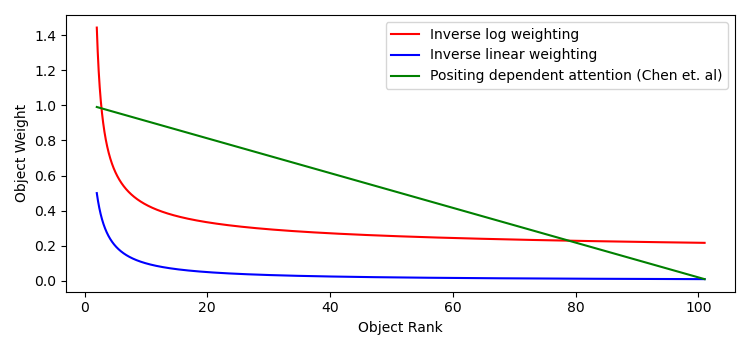
\includegraphics[scale=0.3]{images/weightingfunctions}
    \caption{Different Weighting Functions.}
    \label{fig:weightingfunctions}
\end{figure}
We use Inverse logarithmic weighting.

\end{frame}





\section{Proposed Method: Surrogate Design}

\begin{frame}

\centering
\LARGE{Proposed Method: Surrogate Design}

\end{frame}

\begin{frame}[t]{Basic Ranker}

A basic ranker is a Deep Neural Network that outputs a score and its corresponding rank.

\begin{figure}[htb]
\centering
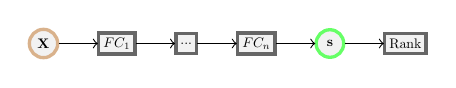
\begin{tikzpicture}[scale=0.50, transform shape,
roundnode/.style={circle, draw=brown!60, fill=black!5, very thick, minimum size=7mm},
roundnodey/.style={circle, draw=green!60, fill=black!5, very thick, minimum size=7mm},
squarednode/.style={rectangle, draw=black!60, fill=black!5, very thick, minimum size=5mm},
]
%Nodes
\node[roundnode]      (X)                             {$\textbf{X}$};
\node[squarednode]      (FC1)                      [right=of X]        {$FC_1$};
\node[squarednode]      (FCmiddle)             [right=of FC1]        {...};
\node[squarednode]      (FCn)                      [right=of FCmiddle]        {$FC_n$};
\node[roundnodey]      (y)                             [right=of FCn] {$\textbf{s}$};
\node[squarednode]      (Rank)                      [right=of y]        {Rank};

%Lines
\draw[->] (X.east) -- (FC1.west);
\draw[->] (FC1.east) -- (FCmiddle.west);
\draw[->] (FCmiddle.east) -- (FCn.west);
\draw[->] (FCn.east) -- (y.west);
\draw[->] (y.east) -- (Rank.west);
\end{tikzpicture}
\caption{Basic ranker.}
\label{fig:basicScoringModel}
\end{figure}

Given a set of inputs $\textbf{X}$,  the ranker outputs the following values
\begin{itemize}
\item Output (or) relevance scores of input elements.  The values are in the \textbf{Output Space}.
\item Ranks of the input elements.  The values are in the \textbf{Ranking Space}.
\end{itemize}

Note:
\begin{itemize}
\item Normal Loss functions work in the Output Space.
\item Ranking Loss functions work in the Ranking Space.
\end{itemize}

\end{frame}


\begin{frame}[t]{Basic Ranker}

A basic ranker is a Deep Neural Network that outputs a score and its corresponding rank.

\begin{figure}[htb]
\centering
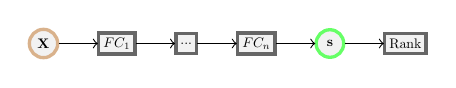
\begin{tikzpicture}[scale=0.50, transform shape,
roundnode/.style={circle, draw=brown!60, fill=black!5, very thick, minimum size=7mm},
roundnodey/.style={circle, draw=green!60, fill=black!5, very thick, minimum size=7mm},
squarednode/.style={rectangle, draw=black!60, fill=black!5, very thick, minimum size=5mm},
]
%Nodes
\node[roundnode]      (X)                             {$\textbf{X}$};
\node[squarednode]      (FC1)                      [right=of X]        {$FC_1$};
\node[squarednode]      (FCmiddle)             [right=of FC1]        {...};
\node[squarednode]      (FCn)                      [right=of FCmiddle]        {$FC_n$};
\node[roundnodey]      (y)                             [right=of FCn] {$\textbf{s}$};
\node[squarednode]      (Rank)                      [right=of y]        {Rank};

%Lines
\draw[->] (X.east) -- (FC1.west);
\draw[->] (FC1.east) -- (FCmiddle.west);
\draw[->] (FCmiddle.east) -- (FCn.west);
\draw[->] (FCn.east) -- (y.west);
\draw[->] (y.east) -- (Rank.west);
\end{tikzpicture}
\caption{Basic ranker.}
\label{fig:basicScoringModel}
\end{figure}

Advantages of working in the ranking space:
\begin{itemize}
\item Ranking is agnostic to affine transformations of score i.e $\alpha * s + \beta$ where $\alpha, \beta \in \mathbb{R}$.
\item Larger target output space leads to easier convergence / learning.
\item Ranks from different rankers can be combined easily.
\end{itemize}

\end{frame}

\begin{frame}[t]{Ensemble of Basic Rankers}

\begin{figure}[htb]
\centering
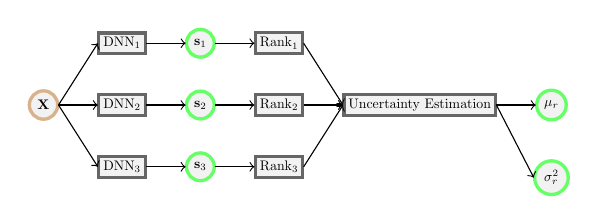
\begin{tikzpicture}[scale=0.50, transform shape,
roundnode/.style={circle, draw=brown!60, fill=black!5, very thick, minimum size=7mm},
roundnodey/.style={circle, draw=green!60, fill=black!5, very thick, minimum size=7mm},
squarednode/.style={rectangle, draw=black!60, fill=black!5, very thick, minimum size=5mm},
]
%Nodes
\node[roundnode]          (X)                                           {$\textbf{X}$};
\node[squarednode]      (DNN2)                      [right=of X]        {DNN$_2$};
\node[squarednode]      (DNN1)                      [above=of DNN2]                    {DNN$_1$};
\node[squarednode]      (DNN3)                      [below=of DNN2]                    {DNN$_3$};
\node[roundnodey]        (y1)                             [right=of DNN1] {$\textbf{s}_1$};
\node[roundnodey]        (y2)                             [right=of DNN2] {$\textbf{s}_2$};
\node[roundnodey]        (y3)                             [right=of DNN3] {$\textbf{s}_3$};
\node[squarednode]      (Rank1)                             [right=of y1] {Rank$_1$};
\node[squarednode]      (Rank2)                             [right=of y2] {Rank$_2$};
\node[squarednode]      (Rank3)                             [right=of y3] {Rank$_3$};
\node[squarednode]      (UncertaintyEstimation)                             [right=of Rank2] {Uncertainty Estimation};
\node[roundnodey]        (mus)                             [right=of UncertaintyEstimation] {$\mu_r$};
\node[roundnodey]        (sigmas)                             [below=of mus] {$\sigma^2_r$};

%Lines
\draw[->] (X.east) -- (DNN1.west);
\draw[->] (X.east) -- (DNN2.west);
\draw[->] (X.east) -- (DNN3.west);
\draw[->] (DNN1.east) -- (y1.west);
\draw[->] (DNN2.east) -- (y2.west);
\draw[->] (DNN3.east) -- (y3.west);
\draw[->] (y1.east) -- (Rank1.west);
\draw[->] (y2.east) -- (Rank2.west);
\draw[->] (y3.east) -- (Rank3.west);
\draw[->] (Rank1.east) -- (UncertaintyEstimation.west);
\draw[->] (Rank2.east) -- (UncertaintyEstimation.west);
\draw[->] (Rank3.east) -- (UncertaintyEstimation.west);
\draw[->] (UncertaintyEstimation.east) -- (mus.west);
\draw[->] (UncertaintyEstimation.east) -- (sigmas.west);

\end{tikzpicture}
\caption{Ensemble of Basic Rankers.}
\label{fig:proposeModelUncertainty}
\end{figure}

\begin{itemize}
\item Ensemble of Basic rankers gives a list of ranks for every input element.
\item Gaussian uncertainty is calculated in the ranking space.. The mean and standard deviation are calculated using the following formulae:
$$
\mu_r = \frac{ \sum\limits_{i=1}^{m} y_i}{m}  \;\;\;\;\;  \sigma_r =\frac{ \sum\limits_{i=1}^{m} (y_i - y_{mean})^2}{m}
$$
\end{itemize}

\end{frame}

\begin{frame}[t]{Making model context aware}



\end{frame}

\section{Testing and Ablation study}

\begin{frame}[t]{Testing and Ablation study}

\end{frame}

\section{Results}
\begin{frame}[t]{Results}
\end{frame}


\section{Discussion}
\begin{frame}[t]{Discussion}

\end{frame}

\section{Q \& A}

\begin{frame}[t]{Q \& A}
  \centering \Huge
  \emph{Q \& A}
\end{frame}

\section{References}

\begin{frame}[t]{References}

\begin{thebibliography}{1}

\bibitem{DeepEnsemblesPaper}
\alert{Balaji Lakshminarayanan and Alexander Pritzel and Charles Blundell; Simple and Scalable Predictive Uncertainty Estimation using Deep Ensembles (2017)}

\end{thebibliography}

\end{frame}

\section{Appendix}

\begin{frame}[t]{Appendix}

\end{frame}

\end{document}
